\chapter{Mechanik}
	\fancyfoot[C]{Kaltenleitner}
	\section{Mechanischer Aufbau}

	Bei dem mechanischen Aufbau von Athena sind viele Faktoren zu beachten. Ein paar dieser Faktoren w�ren der Verwendungszweck, Kosten und die Belastbarkeit. Ebenfalls gibt es auch Modellautos, welche ihre Funktion und Stabilit�t schon am Markt bewiesen haben. Da alle bereits existierenden Fahrzeuge die hohen platztechnischen Anspr�che eines solchen Projekts nicht vollst�ndig erf�llen, ist es besser, das Fahrzeug von Grund auf selbst zu konstruieren. Ein Fahrzeug mit hoher Karosserie ist von Vorteil, da ein solches viel Platz bietet.\\
\\
	F�r den mechanischen Aufbau stehen viele Materialien mit unterschiedlichen Eigenschaften und Preisen zur Verf�gung. Auch kann man sich an Teilen von bereits vorhandenen Fahrzeugen bedienen. Dies wurde im Falle von Athena auch getan. So werden mehrere Teile aufgrund der hohen Kosten im Falle der Eigenanfertigung vom etablierten Modell "X-MAXX" der Firma Traxxas genutzt. Diese Teile umfassen die Lager, D�mpfer und gro�e Teile des Antriebsstrangs. Aufgrund der �bernommenen Komponenten hat man einen gewissen Rahmen, in dem sich bei der Auslegung der Gesamtgr��e bewegen muss. Die Bauteile, die hierbei am meisten ausmachen, sind die Grundplatte und die zentrale Antriebswelle.

\subsection{Grundlegender Aufbau / Montagereihenfolge}
\subsubsection{Antriebsstrang}
	Beim Zusammenbau von Athena wird der Antriebsstrang als erstes montiert. Seine Hauptaufgabe besteht darin, die Leistung vom Motor auf die Reifen zu �bertragen. Der Allradantrieb setzt sich aus drei Differenzialen zusammen. Bei der Konstruktion m�ssen die Abst�nde zwischen dem Kegelrad (gro�es Zahnrad des Differentials) und dem Ritzel ber�cksichtigt werden. Wenn diese nicht passen, kann dies dazu f�hren, dass die Zahnr�der bei hoher Belastung leichter besch�digt werden. Es ist wichtig, beim Zusammenbau auf die Schmierung des Getriebes und der Differenziale zu achten.
		
		\begin{figure}[H]
			\centering
			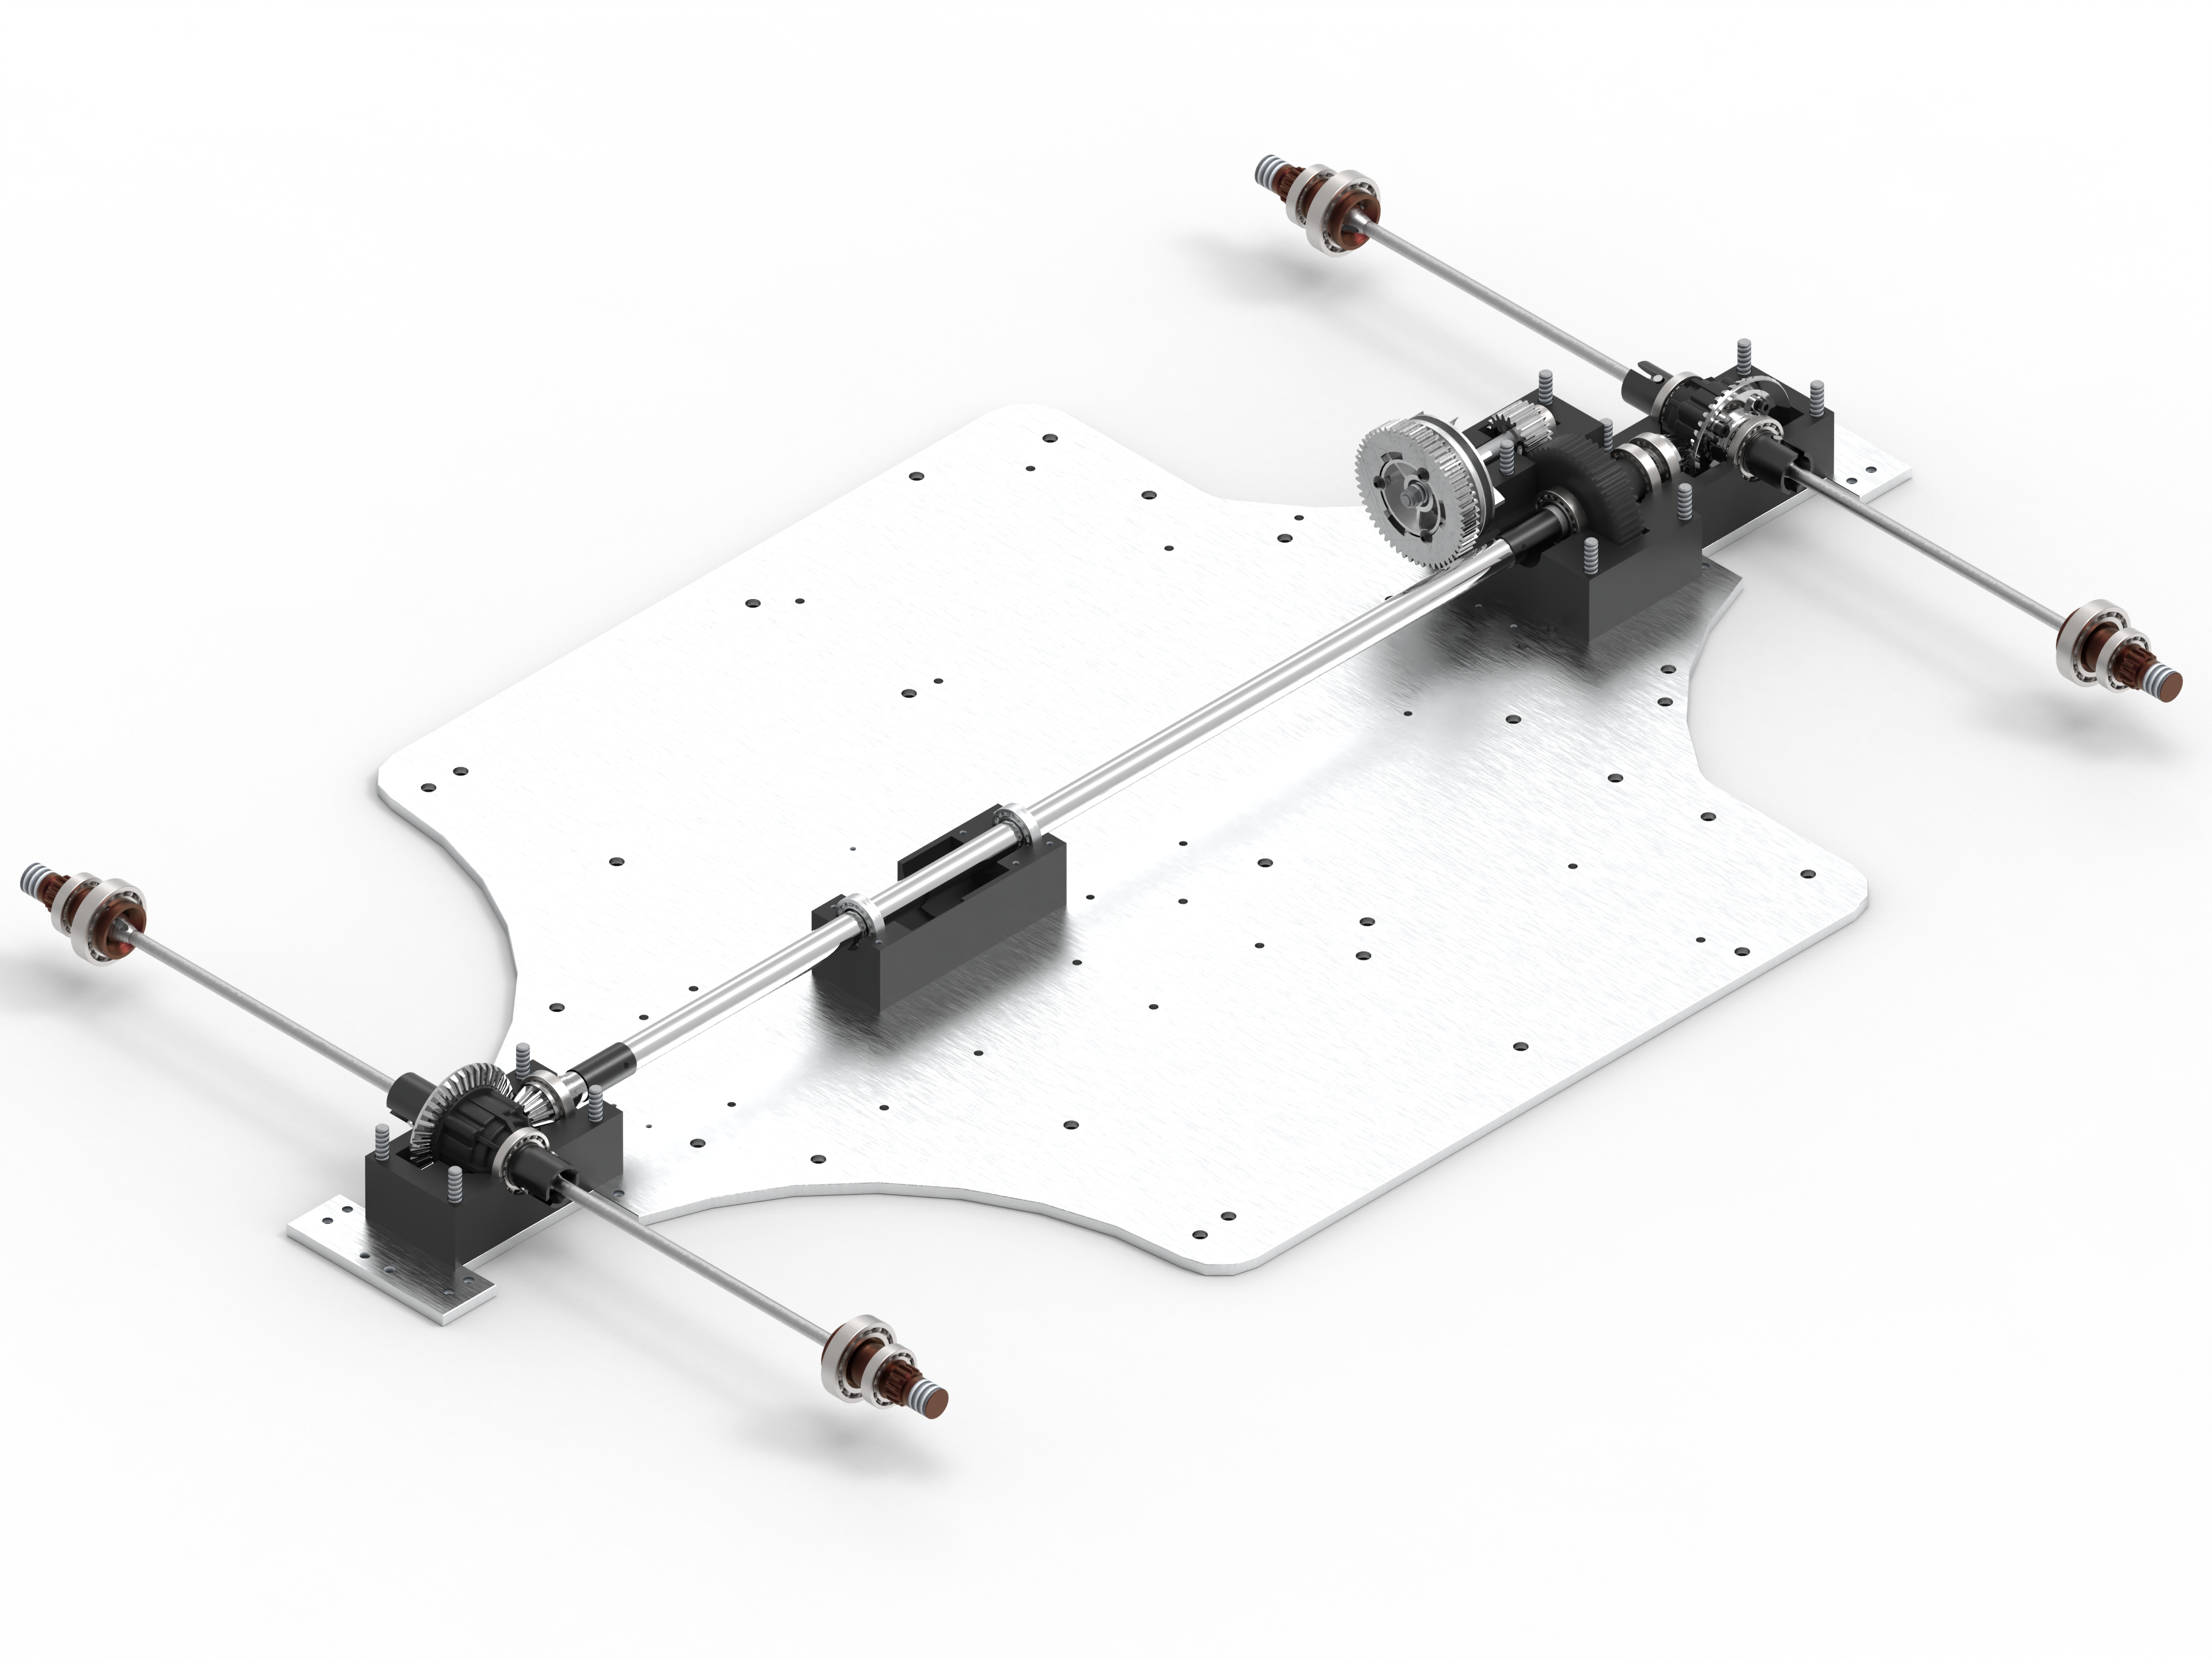
\includegraphics[scale=2.4]{./4_Mechanik/Abbildungen/Aufbau_Anleitung_render/Antriebsstrang_1}
			\caption{ Antriebsstrang ohne obere Getriebegeh�use}
		\end{figure}